\subsection{Silicon vertex tracker {\it Tim}}
\label{sec:svtŧ}


\subsubsection{Sensor Modules}

The sensor modules for the SVT consist of a pair of identical half-modules, sandwiched back-to-back around an aluminum cooling block at one end and a similar PEEK spacer block at the other. Figure \ref{fig:tracker_module} shows a prototype module assembly.
\begin{figure}[ht]
    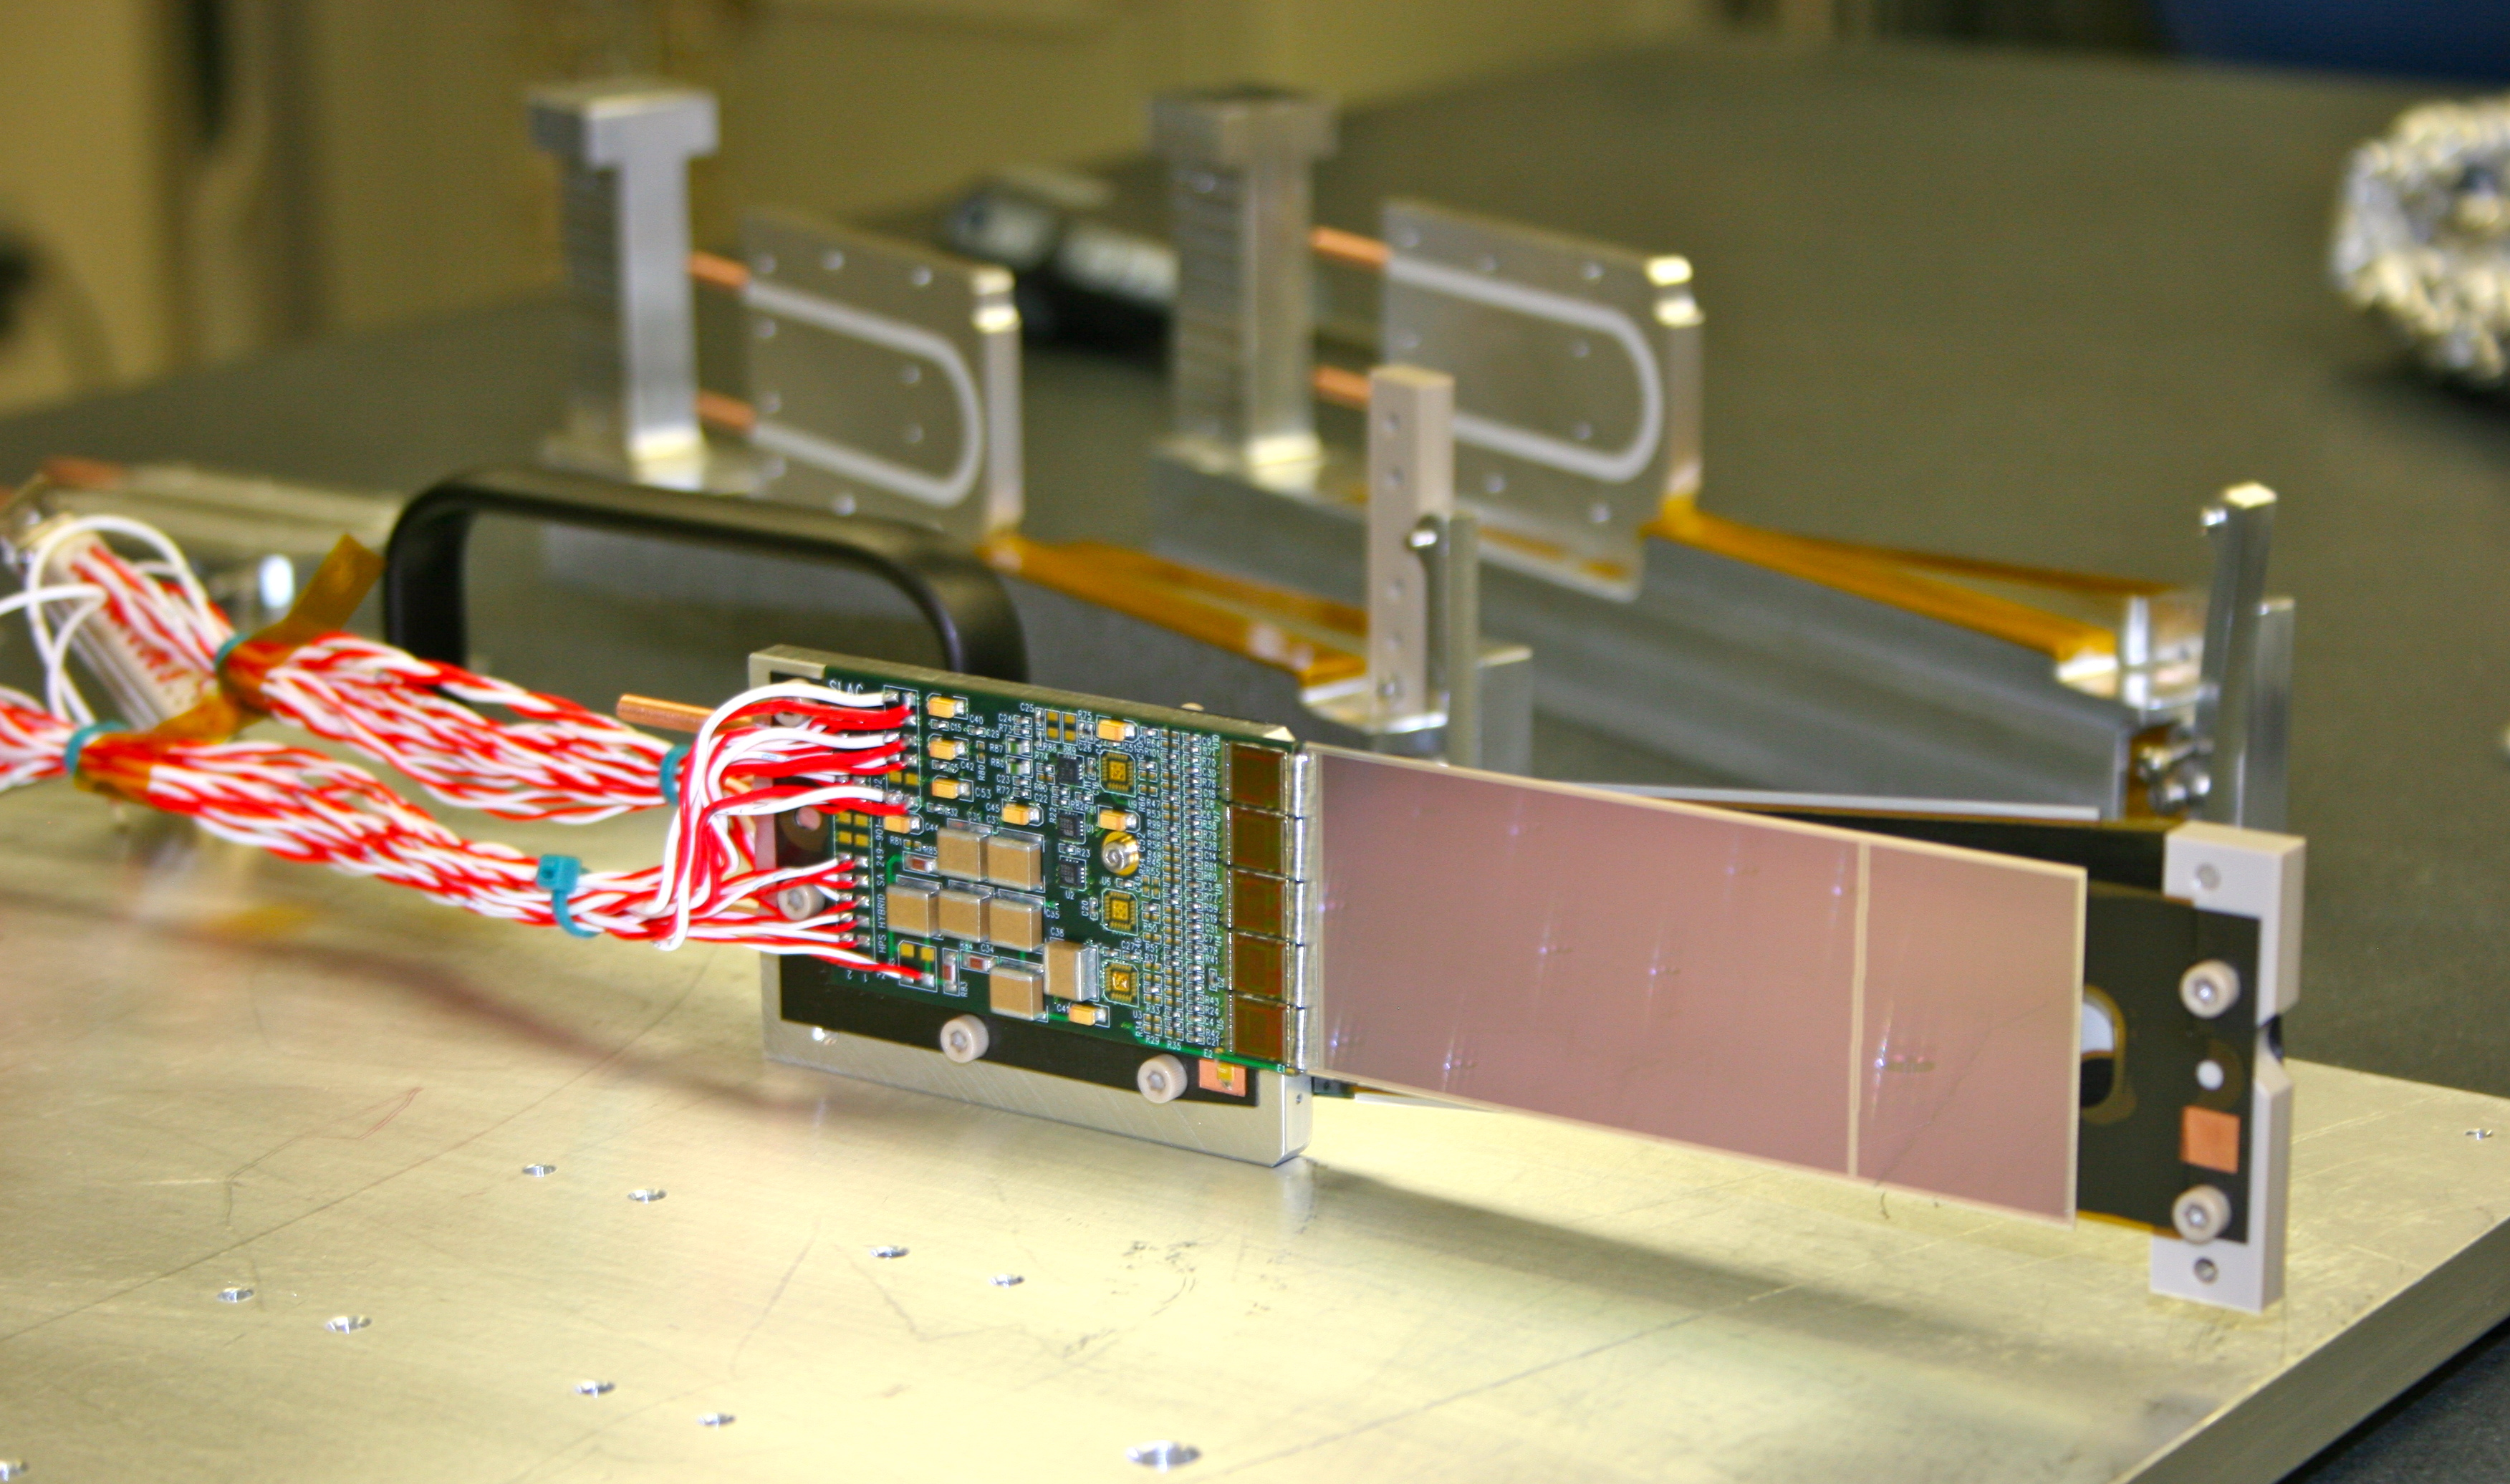
\includegraphics[width=\textwidth]{svt/IMG_5200}
\caption{\small{A prototype module assembly (foreground) with the 50 mrad (left) and 100 mrad (right) module assembly fixtures in the background.  A pair of cooling blocks and a spacer block can be seen on the fixtures.} }
\label{fig:tracker_module}
\end{figure}
The cooling block provides the primary mechanical support for the module as well as cooling via copper tubes pressed into grooves in the plates. The spacer block defines the spacing between the sensors at the far end of the module, stiffens the module structure, and improves the stability of the sensor alignments.  

Each half module consists of a single sensor and a hybrid electronic readout board glued to a polyamide-laminated carbon fiber composite backing.  A window is machined in the carbon fiber leaving only a frame around the periphery of the silicon to minimize material. A 50 $\mu$m sheet of polyamide is laminated to the surface of the carbon fiber with 1 mm overhang at all openings to ensure good isolation between the backside of the sensor, carrying high-voltage bias, and the carbon fiber which is held near ground.  The average support material in the tracking volume is approximately 0.1\% $X_{0}$ per double-sided module.

The sensors are 320 $\mu$m thick, p$^+$ on n-bulk, $<$100$>$, single-sided microstrip sensors manufactured by the Hamamatsu Photonics Corporation for production of layers 2-5 of the D$\O$ Run IIb silicon tracker. Of 33 sensors provided for the SVT, 29 had breakdown voltages in excess of 1000V and all but 4 had no bad channels.  

The readout ASICs are the APV25 readout chip designed for the CMS experiment at the LHC.  In addition to fast readout capability and high radiation tolerance, the APV25 is capable of delivering multiple samples of the amplifier output at a specified pipeline latency which allows asynchronous use of the chip as well as the ability to reconstruct hit time to 2 ns at our high signal-to-noise ratios \cite{HPS_PROP}. Each 10-layer, polyamide hybrid readout board hosts a set of five APV25 and provides conditioned high-voltage for biasing the sensor. Power, control and data for the hybrids are connected via 30 lines of twisted pair wire: an 18~cm ``pigtail'' cable is soldered directly to the surface of the hybrid.  Bias is provided to both top and back side via wire bonds which are also used to connect the front end reference to the carbon fiber. All wire bonds are encapsulated to prevent damage.

Module yields were good for such a small production.  Of 165 chips acquired, 150 were used to assemble 30 production hybrids, of which 29 passed QA testing.  Of 29 modules built, 28 passed QA testing, leaving 8 spare modules after completion of the HPS Test SVT.
